\subsection{Introductie} \label{sec:introduction}
% what is pathloss
% When designing wireless electronic systems, end users usually ask for the estimated range of the system. There are two ways that such an estimate can be obtained. The seemingly most simple one of these methods is to just do some measurements. This method is however not able to produce reliable estimates, unless the system has been tested in lots of different environments. The second method on the other hand is centered around equations that predict the signal degradation over distance. This method is also not a perfect prediction thus requiring a fitting coefficient.

Met de opkomst van IoT (Internet of Things) systemen wordt er steeds vaker verlangd dat elektronische systemen draadloos kunnen communiceren. Het benodigde draadloze bereik van een IoT apparaat is erg afhankelijk van de toepassing. In het geval van een medisch oproep systeem dat enkel binnen één kamer in een verpleeghuis hoeft te werken zal het draadloze bereik niet veel groter hoeven te zijn dan enkele tientallen meters. Echter, wanneer de toepassing in de agrarische sector valt kan een groter bereik van enkele kilometers kilometers gewenst zijn. 

Om ervoor te zorgen dat een IoT systeem niet onnodig veel energie verbruikt, is het belangrijk om ervoor te zorgen dat het draadloze communicatie bereik niet vele malen groter is dan nodig. Door signaalverliezen goed te modelleren kan er een ondergrens gevonden worden voor het minimaal benodigde zendvermogen in een draadloos communicatiesysteem.

In dit meetrapport zal er gekeken worden naar een model om signaalverliezen te modelleren in het Jacoba Mulder Huis, dat op de 
Amstelcampus van de Hogeschool van Amsterdam staat. Het model dat wordt gebruikt in dit meetrapport maakt gebruik van een fittingscoëfficiënt die door middel van metingen zal worden vastgesteld.
% bij IoT systemen erg wisselend wat het nodige bereik van het draadloze netwerk is. Om ervoor te zorgen dat een draadloos systeem een minimaal bereik heeft moet er rekening gehouden worden met signaalverliezen. Een van deze verliezen is path loss. 

% Opdracht en hebben dus model nodig voor path loss in het JMH
% Specificeer frequentie van interesse

% How to calculate path loss 
\subsubsection{Path loss}
Path loss beschrijft de demping van elektromagnetische golven tussen een zender en een ontvanger. Om deze demping te berekenen, kunnen er verschillende modellen worden gebruikt. In het geval dat de antennes zich in free space bevinden kan \cref{eq:receivedPowerFreeSpace} gebruikt worden om het ontvangen vermogen te berekenen \cite[13]{bensky2019shortRangeWirelessCommunication}. In \cref{eq:receivedPowerFreeSpace} zijn \(P_t\) en \(P_r\) de zend en ontvangst vermogens, \(G_t\) en \(G_r\) zijn respectievelijk de zend- en ontvangstversterkingsfactoren van de zend- en ontvangstantennes, \(\lambda\) is de golflengte en d is de afstand tussen de zend- en ontvangstantennes. 
\begin{equation}\label{eq:receivedPowerFreeSpace}
    P_r=\frac{P_tG_tG_r\lambda^2}{\left(4\pi d\right)^2} \,\,\left[\unit{\watt}\right]
\end{equation}
Het berekenen van ontvangen vermogen kan erg nuttig zijn, op het moment dat het zendvermogen bekend is. In het geval een systeem nog ontworpen moet worden is het zendvermogen echter nog niet bekend, en heeft het niet veel nut om het ontvangstvermogen uit te rekenen. Dit is op te lossen door niet het ontvangstvermogen uit te rekenen maar hoeveel demping er in een signaal optreed. In het geval van \cref{eq:receivedPowerFreeSpace} kan de demping van een signaal berekend worden met \cref{eq:FreeSpacePathLoss}.
% In het ontwerpen van communicatie systemen komt het vaak voor dat men wil weten wat de verzwakking van een signaal is in decibel. De verzwakking van een signaal kan berekend worden door \cref{eq:receivedPowerFreeSpace} te herschrijven naar \cref{eq:FreeSpacePathLoss}.
\begin{equation}\label{eq:FreeSpacePathLoss}
    PL_{FS}=20\log\left(\frac{4\pi d}{\lambda\sqrt{G_tG_r}}\right) \,\,\left[\unit{\decibel}\right]
\end{equation}
Wanneer er (nog) geen antenne gekozen is om te gebruiken in een ontwerp zijn de antenneversterkingsfactoren nog niet bekend. Om dan toch nog een indicatie te kunnen krijgen van het signaal verlies kunnen de ontvangst en zendantennes als isotroop worden verondersteld. Een antenne met isotrope eigenschappen heeft namelijk een antenneversterkingsfactor van 1 \cite{bensky2019shortRangeWirelessCommunication}. Dit is omdat een isotrope antenne in alle richtingen met evenveel vermogen zend \cite{bensky2019shortRangeWirelessCommunication}.
Als de zend en ontvangstantennes als isotroop worden verondersteld volgt uit \cref{eq:FreeSpacePathLoss} \cref{eq:isotropicPathLoss}.
%In het geval dat de antennes die worden gebruikt isotrope eigenschappen\footnote{Antennes met isotrope eigenschappen zenden in alle richtingen met evenveel vermogen.} hebben volgt \cref{eq:isotropicPathLoss} uit \cref{eq:FreeSpacePathLoss}. Dit is omdat een antenne met isotrope eigenschappen een antenne versterking van $1$ heeft \cite{bensky2019shortRangeWirelessCommunication}.
\begin{equation} \label{eq:isotropicPathLoss}
    PL_{FS}=20\log\left(\frac{4\pi d}{\lambda}\right) \,\,\left[\unit{\decibel}\right]
\end{equation}

Het path loss model dat beschreven wordt met \cref{eq:FreeSpacePathLoss} gaat er van uit dat de zend- en ontvangst antennes zich in free space bevinden. Dit is echter niet het geval en het model van \cref{eq:FreeSpacePathLoss} zal aangepast moeten worden om meer niet ideale effecten mee te nemen. Een niet idealiteit die meegenomen kan worden is dat de antennes boven een vlak worden geplaatst. Via het vlak waar de antennes boven staan zal er een reflectie ontstaan. Dit is schematisch getoond in \cref{fig:twoRayModelSchem}. Dit nieuwe model staat bekend in de literatuur als het two ray model \cite{MobileAntenaSystemsHandbookCH2}.
\begin{figure}[h]
    \centering
    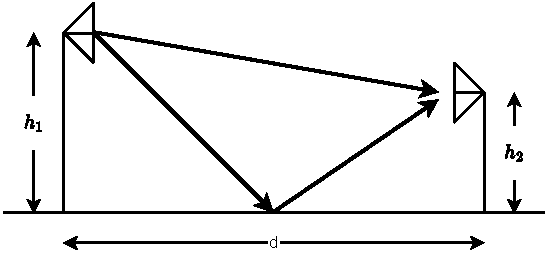
\includegraphics[width=0.6\textwidth]{img/twoRayModel}
    \caption{Het twee stralen model \cite{MobileAntenaSystemsHandbookCH2}.}
    \label{fig:twoRayModelSchem}
\end{figure}

Om het two ray model mee te nemen in de path loss berekening moet er een factor berekend worden. Deze factor moet vervolgens met de uitkomst van het free space path loss model worden vermenigvuldigd. Deze factor wordt gegeven door \cref{eq:twoRayModel} \cite{MobileAntenaSystemsHandbookCH2,brini2019system}. In \cref{eq:twoRayModel} zijn $h_1$ en $h_2$ respectievelijk de hoogtes van antennes 1 en 2, $d$ is de afstand tussen antennes 1 en 2, $\Gamma_\bot$ is de reflectie coefficient en $\beta$ is het golfgetal. het golfgetal kan berekend worden met \cref{eq:calcWaveNumber}. 
\begin{equation}\label{eq:twoRayModel}
    PL_{TR}=-20\log\left[\frac{1}{\left|1+\Gamma_\bot\exp\left[j\beta \left(\sqrt{\left(h_1+h_2\right)^2+d^2}-\sqrt{\left(h_1-h_2\right)^2+d^2}\right)\right]\right|}\right] \,\,\left[\unit{\decibel}\right]
\end{equation}
\begin{equation}\label{eq:calcWaveNumber}
    \beta=\frac{2\pi}{\lambda}
\end{equation}

% Ingaan op de reflectie coefficient.
De reflectie coefficient $\Gamma_\bot$ geeft aan hoeveel vermogen wordt gereflecteerd door de grond. Met \cref{eq:reflectionCoef}, de invalshoek $\theta$ en de permeabiliteit $\epsilon_r$ kan de reflectie coefficient $\Gamma_\bot$ worden berekend \cite{bacco2014uavs,sommer2012applicability}.
\begin{equation}\label{eq:reflectionCoef}
    \Gamma_\bot\left(\theta, \epsilon_r\right)=\frac{\sin\left(\theta\right)-\sqrt{\epsilon_r-\cos^2\left(\theta\right)}}{\sin\left(\theta\right)+\sqrt{\epsilon_r-\cos^2\left(\theta\right)}}
\end{equation}
\begin{equation}
    \theta=\arctan\left(\frac{h_1+h_2}{d}\right)\,\,\unit{\left[rad\right]}
\end{equation}

% Ingaan op vereenvoudiging en waarom die niet gebruikt kan worden voor ons.
In het geval $h_1+h_2\ll d$ kan \cref{eq:twoRayModel} vereenvoudigd worden naar \cref{eq:simplifiedEquation} \cite{brini2019system}.
\begin{equation}\label{eq:simplifiedEquation}
    PL_{TR}=-20\log\left[2\sin\left(\frac{2\pi h_th_r}{\lambda d}\right)\right] \,\,\left[\unit{\decibel}\right]
\end{equation}

De voorgaande modellen zijn niet compleet genoeg om de situatie in een bebouwd gebied te voorspellen. Om een beter model te krijgen kan er een fittings factor worden toegevoegd aan \cref{eq:FreeSpacePathLoss} \cite[24]{brini2019system}. \autoref{eq:fittingFactor} toont deze fittings factor waarin \(l_f\) een fittings coefficient is en $d$ de afstand tussen de twee antennes. \autoref{eq:calcPathLoss} toont de vergelijking van het uitgebreidere model van de path loss.
\begin{equation} \label{eq:fittingFactor}
    F_f=l_f\log(50d) \,\,\left[\unit{\decibel}\right]
\end{equation}
\begin{equation}\label{eq:calcPathLoss}
    PL= PL_{FS}+PL_{TR}+F_l \,\,\left[\unit{\decibel}\right]
\end{equation}

% How to calculate the pathloss fitting coefficient
